\documentclass[12pt]{report}
\usepackage[utf8]{inputenc}
\usepackage[english, russian]{babel}
\usepackage{listings}
\usepackage{graphicx}
\usepackage{float}
\graphicspath{{imgs/}}
\usepackage{amsmath,amsfonts,amssymb,amsthm,mathtools} 
\usepackage{pgfplots}
\usepackage{filecontents}
\usepackage{indentfirst}
\usepackage{eucal}
\usepackage{enumitem}
\frenchspacing
\usepackage{caption}

\usepackage{indentfirst} % Красная строка

\usetikzlibrary{datavisualization}
\usetikzlibrary{datavisualization.formats.functions}

\usepackage{amsmath}
\usepackage{fixltx2e}


\definecolor{bluekeywords}{rgb}{0,0,1}
\definecolor{greencomments}{rgb}{0,0.5,0}
\definecolor{redstrings}{rgb}{0.64,0.08,0.08}
\definecolor{xmlcomments}{rgb}{0.5,0.5,0.5}
\definecolor{types}{rgb}{0.17,0.57,0.68}

\usepackage{listings}
\lstset{language=[Sharp]C,
	captionpos=t,
	numbers=left, %Nummerierung
	numberstyle=\small, % kleine Zeilennummern
	frame=single, % Oberhalb und unterhalb des Listings ist eine Linie
	stepnumber=1,                   
	numbersep=5pt,                
	showspaces=false,
	tabsize=2,
	showtabs=false,
	breaklines=true,
	showstringspaces=false,
	breakatwhitespace=true,
	escapeinside={(*@}{@*)},
	commentstyle=\color{greencomments},
	morekeywords={partial, var, value, get, set},
	keywordstyle=\color{bluekeywords},
	stringstyle=\color{redstrings},
	basicstyle=\ttfamily\small,
}

\usepackage[left=2cm,right=2cm, top=2cm,bottom=2cm,bindingoffset=0cm]{geometry}
% Для измененных титулов глав:
\usepackage{titlesec, blindtext, color} % подключаем нужные пакеты
\definecolor{gray75}{gray}{0.75} % определяем цвет
\newcommand{\hsp}{\hspace{20pt}} % длина линии в 20pt
% titleformat определяет стиль
\titleformat{\chapter}[hang]{\Huge\bfseries}{\thechapter\hsp\textcolor{gray75}{|}\hsp}{0pt}{\Huge\bfseries}


% plot
\usepackage{pgfplots}
\usepackage{filecontents}
\usetikzlibrary{datavisualization}
\usetikzlibrary{datavisualization.formats.functions}
 
\begin{document}
  %\def\chaptername{} % убирает "Глава"
\thispagestyle{empty}
\begin{titlepage}
	\noindent \begin{minipage}{0.15\textwidth}
	
\includegraphics[width=\linewidth]{b_logo}
	\end{minipage}
	\noindent\begin{minipage}{0.9\textwidth}\centering
		\textbf{Министерство науки и высшего образования Российской Федерации}\\
		\textbf{Федеральное государственное бюджетное образовательное учреждение высшего образования}\\
		\textbf{~~~«Московский государственный технический университет имени Н.Э.~Баумана}\\
		\textbf{(национальный исследовательский университет)»}\\
		\textbf{(МГТУ им. Н.Э.~Баумана)}
	\end{minipage}
	
	\noindent\rule{18cm}{3pt}
	\newline\newline
	\noindent ФАКУЛЬТЕТ $\underline{\text{«Информатика и системы управления»}}$ \newline\newline
	\noindent КАФЕДРА $\underline{\text{«Программное обеспечение ЭВМ и информационные технологии»}}$\newline\newline\newline\newline\newline\newline\newline\newline\newline\newline\newline
	
	
	\begin{center}
		\noindent\begin{minipage}{1.3\textwidth}\centering
			\Large\textbf{  Отчет по лабораторной работе №3}\newline
			\textbf{по дисциплине "Анализ алгоритмов"}\newline\newline
		\end{minipage}
	\end{center}
	
	\noindent\textbf{Тема} $\underline{\text{Анализ алгоритмов сортировки}}$\newline\newline
	\noindent\textbf{Студент} $\underline{\text{Малышев И. А.}}$\newline\newline
	\noindent\textbf{Группа} $\underline{\text{ИУ7-51Б}}$\newline\newline
	\noindent\textbf{Оценка (баллы)} $\underline{\text{~~~~~~~~~~~~~~~~~~~~~~~~~~~}}$\newline\newline
	\noindent\textbf{Преподаватель: } $\underline{\text{Волкова Л. Л.}}$\newline\newline\newline
	
	\begin{center}
		\vfill
		Москва~---~\the\year
		~г.
	\end{center}
\end{titlepage}


\renewcommand{\contentsname}{Содержание}
\tableofcontents
  
\newpage
\chapter*{Введение}
\addcontentsline{toc}{chapter}{Введение}


Сортировка является одной из важнейших задач обработки информации. Под сортировкой понимают процесс упорядочивания элементов по какому-либо признаку в заданном массиве элементов. Например, текстовые данные можно отсортировать в лексикографическом порядке, а числовые в порядке неубывания или невозрастания.

В настоящее время многие программные системы работают с большим объёмом данных, поэтому возникает задача ускорения процесса обработки. Именно эту задачу и решают алгоритмы сортировки. Так, время поиска в отсортированном массиве пропорционально логарифму количества элементов, а в неотсортированном - пропорционально количеству элементов, что значительно медленнее.

Важной характеристикой любого алгоритма сортировки является скорость его работы, то есть время, за которое данные будут отсортированы. Время сортировки будет зависеть от количества сравнений и перестановок элементов, а также от длины массива данных. 

Поэтому \textbf{целью} данной работы является получить навыки сравнительного анализа на примере 3 алгоритмов сортировки: сортировки пузырьком, сортировки выбором и быстрой сортировки. 

Для достижения поставленной цели необходимо решить следующие \textbf{задачи}:
\begin{itemize}
\item изучить алгоритмы сортировки;
\item провести сравнительный анализ алгоритмов на основе теоретических расчётов;
\item реализовать алгоритмы сортировки;
\item протестировать реализованные алгоритмы;
\item провести сравнительный анализ реализаций алгоритмов по затраченному процессорному времени.
\end{itemize}


\chapter{Аналитическая часть}

В этом разделе приведён обзор и анализ алгоритмов сортировки.

\section{Сортировка пузырьком}

Алгоритм состоит из последовательных проходов по массиву. За один проход элементы всех пар стоящих рядом элементов сравнивают друг с другом и, если они стоят в неверном порядке, меняют их местами. Проходы повторяются $N - 1$ раз, где $N$ - длина массива. При каждом проходе алгоритма по внутреннему циклу очередной наибольший элемент массива ставится на свое место в конце массива рядом с предыдущим ``наибольшим элементом'', а наименьший элемент массива перемещается на одну позицию к началу массива (``всплывает'' до нужной позиции, как пузырёк в воде -- отсюда и название алгоритма).

Из описания алгоритма очевидна модификация, ускоряющая его: если за проход не было обменов, то все элементы стоят на своих местах, следовательно, можно закончить выполнение сортировки (т. н. Сортировка пузырьком с флагом). 

При этом важно заметить, что алгоритм является устойчивым, то есть одинаковые по заданному признаку элементы останутся в том же порядке, что и до сортировки.

\section{Сортировка выбором}

Идея алгоритма заключается в том, что массив делят на 2 части: отсортированную и неотсортированную. Части отделяет текущий элемент. Текущий элемент сравнивают с каждым элементом из неотсортированной части. Среди них находят минимальный элемент, после этого производится обмен местами с текущим элементом и граница смещается на один элемент к концу массива. Алгоритм заканчивается тогда, когда отсортированной частью массива будет являться весь массив. 

Важно заметить, что алгоритм не является устойчивым, т. е. элементы, которым не нужно менять порядок, всё равно будут его менять во время работы алгоритма.

\section{Быстрая сортировка}

Идея алгоритма состоит из трёх действий, описанные ниже.

\begin{enumerate}
	\item Выбрать из массива элемент, называемый опорным. Это может быть любой из элементов массива. От выбора опорного элемента не зависит корректность алгоритма, но может зависеть его эффективность. Обычно выбирают средний элемент.
	\item Сравнить все остальные элементы с опорным и переставить их в массиве так, чтобы разбить массив на два отрезка: «меньшие опорного» и «равные и большие».
	\item Для двух отрезков рекурсивно применяем ту же последовательность действий, пока длина отрезка больше единицы.
\end{enumerate}

\section{Вывод}

В данном разделе были описаны идеи трёх алгоритмов сортировки: сортировки пузырьком, выбором и быстрой сортировки.
	
\newpage

\chapter{Конструкторская часть}

В этом разделе приводятся схемы алгоритмов сортировки, приведённых в аналитической части, и расчёты их трудоёмкости. 

\section{Схемы алгоритмов}

На рисунках \ref{bubs}, \ref{sels} и \ref{qsorts} показаны схемы алгоритмов сортировки пузырьком, выбором и быстрой сортировки соответственно.

\begin{figure}[H]
	\raggedleft
	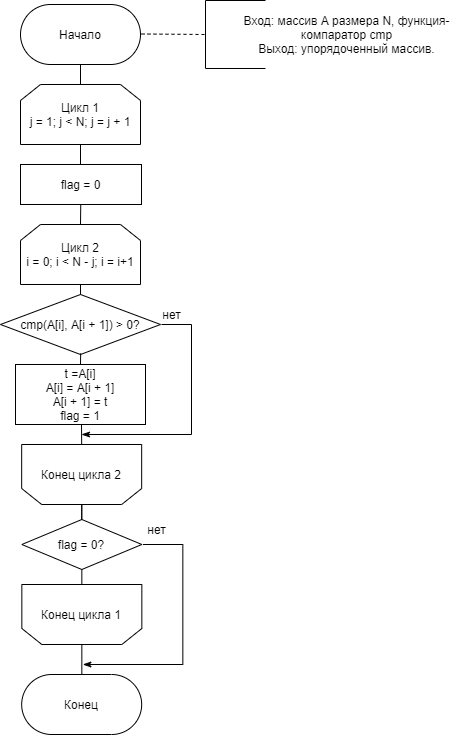
\includegraphics[scale = 0.53]{bsort.png}
	\caption{Схема сортировки пузырьком}
	\label{bubs}
\end{figure}

\begin{figure}[H]
	\raggedleft
	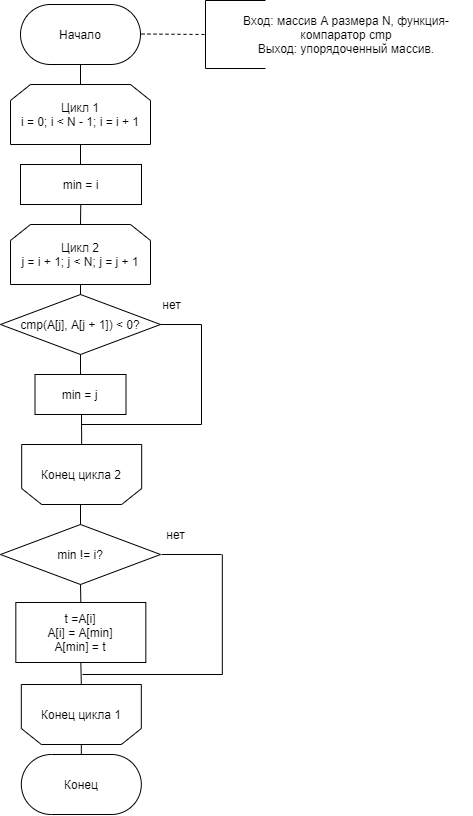
\includegraphics[width=0.75\linewidth]{ssort.png}
	\caption{Схема сортировки выбором}
	\label{sels}
\end{figure}

\begin{figure}[H]
	\raggedleft
	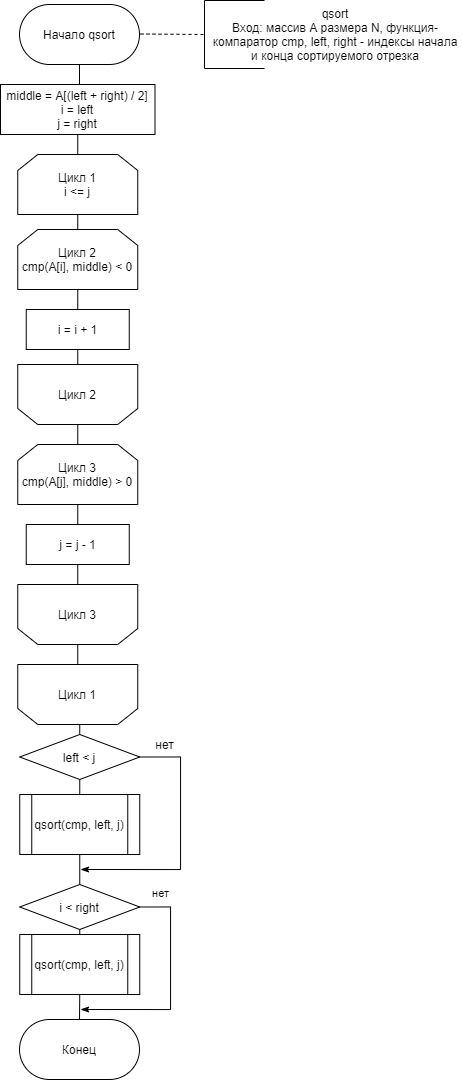
\includegraphics[scale=0.6]{qsort.png}
	\caption{Схема быстрой сортировки}
	\label{qsorts}
\end{figure}



\section{Трудоемкость алгоритмов}
Введем модель трудоемкости для оценки алгоритмов:
\begin{enumerate}
  	\item  базовые операции стоимостью 1: +, -, *, /, =, ==, <=, >=, !=, +=, [], получение полей класса;
	\item оценка трудоемкости цикла: F\textsubscript{ц} = a + N * (a + F\textsubscript{тела}), где a - условие цикла;
	\item стоимость условного перехода возьмем за 0, стоимость вычисления условия остаётся.
\end{enumerate}

Далее будет приведены оценки трудоемкости алгоритмов. 

\subsection{Сортировка пузырьком с флагом}
Построчная оценка трудоемкости сортировки пузырьком с флагом (Табл. 2.1).
\begin{center}
Табл. 2.1 Построчная оценка трудоемкости для алгоритма сортировки пузырьком с флагом

	\begin{tabular}{|l c|} 
 	\hline
	Код & Вес \\ [0.5ex] 
 	\hline
	bool flag = false; & 1\\
 	\hline
	for (int i = 1; i < Length; i++) & 3\\
	\hline
	\{ & 0\\
	\hline
	\quad flag = false; & 1\\
 	\hline
	\quad for (int j = 0; j < Length - i; j++) & 4\\
	\hline
	\quad \{ & 0\\	
	\hline
	\quad \quad if(arr[i] < arr[i + 1]) & 4\\
	\hline
	\quad \quad \{ & 0\\
	\hline
	\quad \quad \quad tmp = arr[i]; & 2\\
	\hline
    \quad \quad \quad arr[i] = arr[i + 1]; & 3\\
    \hline
    \quad \quad \quad arr[i + 1] = tmp; & 2\\
    \hline
    \quad \quad \quad flag = true; & 1\\
    \hline
    \quad \quad \} & 0\\
	\hline
	\quad \} & 0\\
	\hline
	\quad if (flag == false) break;  & 1\\
	\hline
	\} & 0\\
	\hline
	\end{tabular}
\end{center}

 
\textbf{Лучший случай:} Массив отсортирован; не произошло ни одного обмена за 1 проход -> выходим из цикла \newline
Трудоемкость:  $1 + 2 + 1 * (1 + 1 + 3 + (n - 1) * (4 + 1) + 1) = 5n + 4 = O(n)$

\textbf{Худший случай:}  Массив отсортирован в обратном порядке; в каждом случае происходил обмен, все внутренние циклы будут состоять из N - j итераций.\newline
Трудоемкость: $1 + 2 + (n - 1) * (1 + 3 + (n - 2) * (1 + 4 + 2 + 3 + 3 + 1) + 1) / 2 = 7n^2 - 18.5n + 14.5 = O(n ^ 2)$
\newline
\newline
\newline
\subsection{Сортировка выбором}
Построчная оценка трудоемкости сортировки выбором (Табл. 2.2).
\begin{center}
Табл. 2.2 Построчная оценка трудоемкости для алгоритма сортировки выбором

	\begin{tabular}{|l c|} 
 	\hline
	Код & Вес \\ [0.5ex] 
 	\hline
 	int min = 0; & 1\\
 	\hline
	for (int i = 0; i < Length - 1; i++) & 4\\
	\hline
	\{ & 0\\
	\hline
	\quad min = i; & 1\\
 	\hline
	\quad for (int j = i + 1; j < arr.Length; j++) & 4\\
	\hline
	\quad \{ & 0\\	
	\hline
	\quad \quad if(arr[j] < arr[min]) & 3\\
    \hline
    \quad \quad \quad min = j; & 1\\
	\hline
	\quad \} & 0\\
	\hline
	\quad if (min != i) & 1\\
	\hline
	\quad \{ & 0\\
	\hline
	\quad \quad tmp = arr[i]; & 2\\
	\hline
    \quad \quad arr[i] = arr[min]; & 2\\
    \hline
    \quad \quad arr[min] = tmp; & 2\\
    \hline
	\quad \} & 0\\
	\hline
	\} & 0\\
	\hline
	\end{tabular}
\end{center}
\hspace*{5mm}


\textbf{Лучший случай:} отсортированный массив, обмены не производятся.
\newline
Трудоемкость: $1 + 3 + (n - 1)(1 + 3 + (n - 2)(1 + 3)) = 4n^2 - 8n + 8 = O(n^2)$
\newline
\hspace*{5mm}
\textbf{Худший случай:} массив отсортирован в обратном порядке, все обмены будут произведены. \newline
Трудоемкость: $1 + 3 + (n - 1)(1 + 3 + (n - 2)(1 + 3 + 1 + 2 + 2 + 2)) = 11n^2 - 29n + 22 = O(n^2)$

\subsection{Быстрая сортировка}
\textbf{Лучший случай:} сбалансированное дерево вызовов \(O(n*log(n))\). 
В cбалансированном варианте при каждой операции разделения массив делится на две одинаковые части, следовательно, максимальная глубина рекурсии, при которой размеры обрабатываемых подмассивов достигнут 1, составит log2n. В результате количество сравнений, совершаемых быстрой сортировкой, равно значению рекурсивного выражения $C_n = 2 * C_{n / 2} + n$, что дает общую сложность O(nlogn) [1].

\textbf{Худший случай:} несбалансированное дерево $O(n^2)$.
В несбалансированном варианте каждое разделение даёт два подмассива размерами 1 и $n - 1$, то есть при каждом рекурсивном вызове больший массив будет на 1 короче, чем в предыдущий раз. В этом случае потребуется $\sum_{{i=0}}^{n}(n-i)=O(n^{2})$ операций, то есть сортировка будет выполняться за квадратичное время [1].

\newpage
\section{Вывод}
На основе описания алгоритмов, данного в аналитическом разделе, были построены схемы трёх алгоритмов сортировки, оценены их трудёмкости в лучшем и худшем случаях. Таким образом, были получены следующие трудоёмкости:
\begin{itemize}
\item сортировка пузырьком: лучший - $O(n)$, худший - $O(n^2)$;
\item сортировка выбором: лучший - $O(n^2)$, худший - $O(n^2)$;
\item быстрая сортировка: лучший - $O(nlogn)$, худший - $O(n^2)$.
\end{itemize}

\newpage
\chapter{Технологическая часть}
В данном разделе приводятся реализации алгоритмов, схемы которых были разработаны в конструкторской части. Кроме того, обосновывается выбор технологического стека и проводится тестирование реализованных алгоритмов.

\section{Средства реализации}

В качестве языка программирования был выбран C\# [2], а среду разработки -- Visual Studio, т. к. я знаком с данным языком и имею представление о тестировании программ в данном языке. Время работы алгоритмов было замерено с помощью библиотеки System.Diagnostics, класса Stopwatch, который имеет методы для расчёта процессорного времени [3].

\section{Входные и выходные данные}
На вход ПО получает массив сравнимых элементов. На выходе -- тот же массив, но отсортированный в заданном порядке.

\section{Реализация алгоритмов}

В листингах 3.1 - 3.3 приведена реализация трёх алгоритмов сортировки.
\captionsetup{singlelinecheck = false, justification=raggedright}
\newpage
\begin{lstlisting}[label=some-code,caption=Функция быстрой сортировки]
static int _Partition(int[] arr, int start, int end)
{
	int p = arr[(end - start) / 2 + start];
	int i = start - 1;
	int j = end + 1;
	
	while (true)
	{
		do i++; while (arr[i] < p);
		do j--; while (arr[j] > p);
		
		if (i >= j) return j;
		
		Swap(ref arr[i], ref arr[j]);
	}
}

static void _QuickSort(int[] arr, int start, int end)
{
	int i;
	if (start < end)
	{
		i = _Partition(arr, start, end);
		
		_QuickSort(arr, start, i);
		_QuickSort(arr, i + 1, end);
	}
}

static void QuickSort(int[] array)
{
	_QuickSort(array, 0, array.Length - 1);
}
\end{lstlisting}
\newpage
\begin{lstlisting}[label=some-code,caption=Функция сортировки массива пузырьком с флагом]
static void BubleFlagSort(int[] arr)
{
	bool flag;
	
	for (int i = 1; i < arr.Length; i++)
	{
		flag = false;
		
		for (int j = 0; j < arr.Length - i; j++)
		{
			if (arr[j] > arr[j + 1])
			{
				Swap(ref arr[j], ref arr[j + 1]);
				flag = true;
			}
		}
		
		if (!flag)
			break;
	}
}
\end{lstlisting}


\begin{lstlisting}[label=some-code,caption=Функция сортировки массива выбором]
static void SelectionSort(int[] arr)
{
	int min;
	
	for (int i = 0; i < arr.Length - 1; i++)
	{
		min = i;
		for (int j = i + 1; j < arr.Length; j++)
			if (arr[j] < arr[min])
				min = j;
		
		if (min != i)
			Swap(ref arr[i], ref arr[min]);
	}
}
\end{lstlisting}
\captionsetup{singlelinecheck = false, justification=centering}
\newpage
\section{Тестирование}

В таблице~\ref{tbl:test} приведены тесты для функций, реализующих алгоритмы сортировки. Все тесты пройдены успешно.

\begin{table}[h!]
	\begin{center}
	\caption{\label{tbl:test}Тестирование реализованных алгоритмов}
		\begin{tabular}{|c|c|c|}
		
			\hline
			Входной массив &  Ожидаемый результат & Фактический результат \\ 
			\hline
			$[-4, -4, -9, 9, 2]$ & $[-9, -4, -4, 2, 9]$  & $[-9, -4, -4, 2, 9]$\\\hline
			$[-5, 6, -1, 5, 8]$  & $[-5, -1, 5, 6, 8]$  & $[-5, -1, 5, 6, 8]$\\\hline
			$[7]$  & $[7]$  & $[7]$\\\hline
			$[]$  & $[]$  & $[]$\\\hline
			$[1, 0, -1]$  & $[-1, 0, 1]$  & $[-1, 0, 1]$\\\hline
		\end{tabular}
		
	\end{center}
\end{table}

\section{Вывод}

В данном разделе были выбраны средства разработки и с помощью них реализованы три алгоритма сортировки: пузырьком, выбором и быстрая сортировка. Кроме того, было проведено тестирование реализованных алгоритмов.

\chapter{Исследовательская часть}

В данном разделе проводится сравненительный анализ реализованных алгоритмов по процессорному времени.

\section{Технические характеристики}

Ниже приведены технические характеристики устройства, на котором было проведено тестирование ПО:

\begin{itemize}
	\item Операционная система: Windows 10 Home 64-bit [4];
	\item Оперативная память: 16 GB;
	\item Процессор: 4.0 GHz 4‑ядерный процессор Intel Core i7-4790K [5].

\end{itemize}

\section{Время выполнения реализаций алгоритмов}

Процессорное время выполнения алгоритма замерялось с помощью класса Stopwatch: для более точного замера каждая сортировка на каждой длине массива выполнялась несколько раз, а затем время усреднялось. 
На рисунках \ref{fig:mpr1}, \ref{fig:mpr2} и \ref{fig:mpr3} показаны зависимости процессорного времени выполнения сортировок от размера массива. Размеры массива варьировались от 100 до 1000. Время приведено в микросекундах. В таблицах \ref{t1}, \ref{t2} и \ref{t3} показано время выполнения алгоритмов в зависимости от размеров массива.

\begin{table} [H]
	\caption{Таблица времени выполнения сортировок на отсортированных данных (в мкс)}
	\label{t1}
	\begin{center}
	\begin{tabular}{|c c c c|}
	\hline
	Размер & bsort & ssort & qsort  \\ [0.5ex]
	\hline
	100 & 1.07 & 37.53 & 6.10  \\ 
	\hline
	200 & 2.02 & 149.26 & 13.07  \\ 
	\hline
	300 & 2.78 & 346.79 & 19.63  \\ 
	\hline
	400 & 3.41 & 603.28 & 26.39  \\ 
	\hline
	500 & 4.25 & 900.45 & 44.86  \\ 
	\hline
	600 & 5.07 & 1279.26 & 41.92  \\ 
	\hline
	700 & 5.92 & 1812.68 & 55.55 \\ 
	\hline
	800 & 6.77 & 2395.87 & 63.59  \\ 
	\hline
	900 & 7.97 & 2965.90 & 81.32 \\
	\hline
	1000 & 7.16 & 3553.72 & 84.51 \\
	\hline 
	\end{tabular}
	\end{center}
\end{table}

\begin{figure}[H]
	\centering
	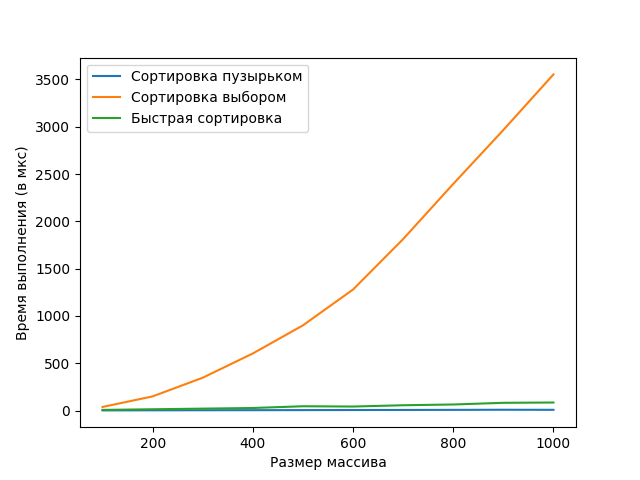
\includegraphics[scale = 0.8]{dir.png}
	\caption{Зависимость времени выполнения сортировок от размера массива на отсортированных данных}
	\label{fig:mpr1}
\end{figure}

\begin{table} [H]
	\caption{Таблица времени выполнения сортировок на отсортированных в  обратном порядке данных (в мкс)}
	\label{t2}
	\begin{center}
	\begin{tabular}{|c c c c|}

		\hline

		Размер & bsort & ssort & qsort \\ [0.5ex]
\hline
100 & 94.97 & 40.37 & 6.40  \\ 
\hline
200 & 430.85 & 138.77 & 13.17  \\ 
\hline
300 & 756.08 & 342.28 & 20.99  \\ 
\hline
400 & 1566.99 & 613.07 & 34.24  \\ 
\hline
500 & 2425.09 & 918.80 & 45.05  \\ 
\hline
600 & 3417.56 & 1242.70 & 49.46  \\ 
\hline
700 & 4512.78 & 1742.92 & 51.72  \\ 
\hline
800 & 5886.49 & 2448.24 & 68.06  \\ 
\hline
900 & 7473.29 & 2983.23 & 85.06 \\
\hline
1000 & 9070.99 & 3681.87 & 89.79 \\
\hline

	\end{tabular}
	\end{center}
\end{table}

\begin{figure}[H]
	\centering
	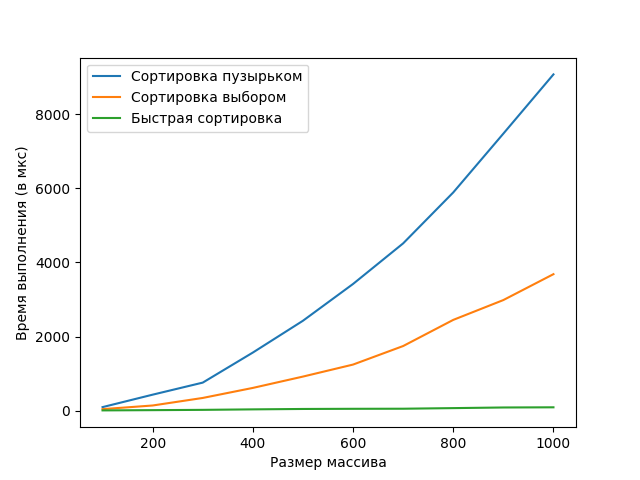
\includegraphics[scale = 0.8]{undir.png}
	\caption{Зависимость времени выполнения сортировок от размера массива на отсортированных в обратном порядке данных}
	\label{fig:mpr2}
\end{figure}

\begin{table} [H]
	\caption{Таблица времени выполнения сортировок на случайных данных (в мкс)}
	\label{t3}
	\begin{center}
	\begin{tabular}{|c c c c|}
		\hline
		Размер & bsort & ssort  & qsort \\ [0.5ex]
		\hline
100 & 78.83 & 44.63 & 7.61  \\ 
\hline
200 & 291.00 & 184.57 & 17.25  \\ 
\hline
300 & 665.56 & 365.30 & 27.60 \\ 
\hline
400 & 1160.13 & 610.15 & 57.50  \\ 
\hline
500 & 1819.05 & 910.41 & 76.51  \\ 
\hline
600 & 2630.66 & 1284.73 & 84.09  \\ 
\hline
700 & 3494.18 & 1806.15 & 132.21  \\ 
\hline
800 & 4617.10 & 2393.96 & 172.21  \\ 
\hline
900 & 5990.72 & 3002.44 & 180.78 \\
\hline
1000 & 7337.07 & 3626.99 & 227.67 \\
\hline

	\end{tabular}
	\end{center}
\end{table}

\begin{figure}[H]
	\centering
	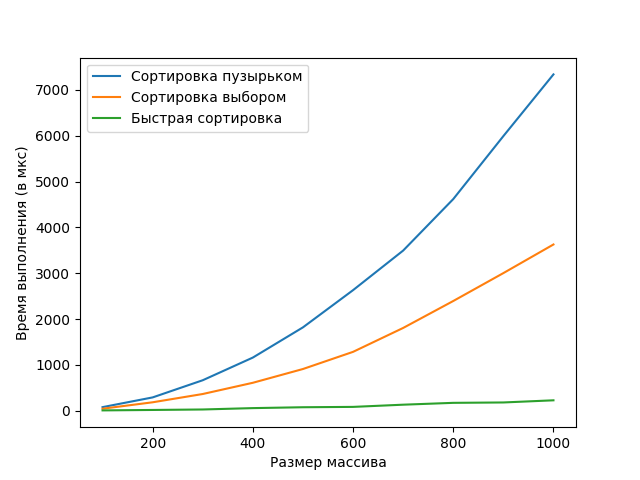
\includegraphics[scale = 0.8]{rand.png}
	\caption{Зависимость времени выполнения сортировок от размера массива на произвольных данных}
	\label{fig:mpr3}
\end{figure}

\section{Вывод}

Как и ожидалось в результате оценки трудоемкости алгоритмов, сортировка пузырьком работает очень быстро на уже отсортированном массиве (лучший случай - оценка O(n)) и очень меделенно на отсортированном в обратном порядке (худший случай - оценка O($n^2$)). Время сортировки выбором на всех трёх видах массивов примерно одинаково, поскольку лучший и худший случаи работают за квадратичное время. Быстрая сортировка работает лучше двух других сортировок на конкретных данных во всех трёх приведённых случаях.


\chapter*{Заключение}
\addcontentsline{toc}{chapter}{Заключение}

В рамках данной лабораторной работы были решены следующие задачи:

\begin{itemize}
	\item изучены 3 алгоритма сортировки: пузырьком, выбором, быстрая сортировка;
	\item реализованы 3 алгоритма сортировки: пузырьком, выбором, быстрая сортировка;
	\item протестированы реализованные алгоритмы;
	\item проведён сравнительный анализ трудоёмкости алгоритмов на основе теоретических расчетов;
	\item проведён сравнительный анализ алгоритмов по затраченному процессорному времени.
\end{itemize}

Цель работы достигнута: получены навыки сравнительного анализа на примере 3 алгоритмов сортировки: сортировки пузырьком, сортировки выбором и быстрой сортировки. 

На основании анализа трудоемкости алгоритмов было показано, что алгоритм сортировки пузырьком имеет наименьшую сложность (линейную) в уже отсортированном массиве и квадратичную в отсортированном обратно, сортировка выбором имеет квадратичную сложность в лучшем, худшем и среднем случаях, а быстрая сортировка работает в лучшем и среднем случае с меньшей сложностью ($O(nlogn)$), чем два других алгоритма, однако при неудачно выбранном опорном элементе и она может достигать квадратичной сложности. Те же выводы были подверждены экспериментально на основе замеров процессорного времени работы алгоритмов. 

\chapter*{Список литературы}
\addcontentsline{toc}{chapter}{Список литературы}
\begin{enumerate}
	\item Кормен Т. Алгоритмы: построение и анализ [Текст] / Кормен Т. - Вильямс, 2014. - 198 с. - 219 с.
	\item Язык программирования C\# [Электронный ресурс]. Режим доступа: https://docs.microsoft.com/ru-ru/dotnet/csharp/. Дата обращения: 02.10.2021
	\item Свойство Process.UserProcessorTime [Электронный ресурс]. Режим доступа: https://docs.microsoft.com/ru-ru/dotnet/api/system.diagnostics.stopwatch?view=net-5.0. Дата обращения: 02.10.2021
	\item Windows 10 [Электронный ресурс]. Режим доступа: https://www.microsoft.com/ru-ru/windows/get-windows-10. Дата обращения: 02.10.2021
	\item Процессор Intel Core I7-4790K [Электронный ресурс]. Режим доступа: https://ark.intel.com/content/www/ru/ru/ark/products/80807/intel-core-i7-4790k-processor-8m-cache-up-to-4-40-ghz.html. Дата обращения: 02.10.2021
	
\end{enumerate}


\end{document}